\chapter{Iterative programming with LLMs}
\label{ch:boptest}

\begin{remark}
  An earlier revision of this chapter was included in a paper~\cite{zabalaComparisonProgramSynthesis2023} presented at SDEWES 2023.
\end{remark}

\section{Motivation}

The chronological order of work that went into this thesis is intentionally kept somewhat secret, but in this case it is too relevant to omit: OpenAI Codex \cite{chenEvaluatingLargeLanguage2021}, the first autoregressive foundation model (section \ref{sec:pretrain}) for program synthesis, was unveiled concurrently with the preparation of chapter \ref{ch:tree2tree}, \emph{prompting} the field to of program synthesis to rethink many (if not most) of its methodological assumptions.
This thesis is no exception.

Codex was \emph{promptly} followed by a wave of instruction fine-tuned models~\cite{zhangInstructionTuningLarge2023} that use human feedback \cite{chaudhariRLHFDecipheredCritical2024, kaufmannSurveyReinforcementLearning2024} in their training process and are designed to explicitly or implicitly admit two inputs: a source text (or code) and a textual command instructing the model to edit the source in a particular way, e.g., ``summarize'' or ``translate to Python.''
These models have been shown to be highly successful in automatic program repair~\cite{fanAutomatedRepairPrograms2023}. 
However, given the free-form nature of these instructions, how one should engineer instructions that maximize repair performance is an open question. 

All the above models, whether instruction-tuned or not, operate in \emph{code translation} paradigm (section \ref{sec:code-translation}), transforming string input into string output.
In contrast with RLCEF (section \ref{sec:rlcef}), this paradigm imposes significant constraints on how the task can be specified.
In particular, it is incompatible with our proposed approach (chapter \ref{ch:proposal}) of using a patient simulator as specification.

The disadvantages of textual \emph{prompts} as the only form of specification are supported by the research literature as well: large language models for code can be very brittle with respect to the input \emph{prompt} \cite{Chen2024NLPerturbator, Erik2022Capturing, Hossen2024On, Shirafuji2023Exploring, Shivagunde2024Deconstructing, Verma2024On, Wang2022ReCode, Zhuo2023On} and display something known as "near-miss syndrome" or "last mile problem" \cite{bavishi2022:neurosymbolic, liuYourCodeGenerated2023, renCodeBLEUMethodAutomatic2020}, i.e. generate solutions that are superficially similar to the desired code, but fail when tested in the real world due to, for example, incorrect input output format.

\newpage
\section{Synthesize, Execute, Debug}
One promising approach to address these limitations and bridge the ``last mile'' is \emph{Synthesize, Execute, Debug}~\cite{guptaSynthesizeExecuteDebug2020}, a framework that introduces program repair into the program synthesis algorithm. 
A programming task is specified using both a natural language description and a set of input/output (I/O) pairs that demonstrate what output is expected from the program, thereby combining text-to-code~\cite{iyer2018:mapping} and programming by example~\cite{halbertProgrammingExample1984,gulwani2016:programming} paradigms typical for competitive programming~\cite{zavershynskyi2018:naps}.
\emph{Synthesize, Execute, Debug} creates a first draft program using a generative model, compiles and executes it with given input examples.
This is followed by a program repair step to fix the identified errors.

The advantages of \emph{Synthesize, Execute, Debug} are two-fold:

\begin{enumerate}
  \item It enables the model to glean additional information from the test environment (such as a patient simulator) that is not included in the initial prompt.
  \item Large Language Model inference normally involves a fixed amount of computation that doesn't depend on the difficulty of the task at hand. Teaching them to iterate enables \emph{test time scaling}~\cite{zhangWhatHowWhere2025}: by changing the number of iterations, the algorithm can scale the computational investment up and down depending on the problem being solved.
\end{enumerate}

This chapter is dedicated to \rqboptest:

\begin{highlight}
  Can \emph{Synthesize, Execute, Debug} with a large language model outperform traditional methods such as model predictive control in a realistic simulated environment?
\end{highlight}

\newpage
\section{Experimental design}
\label{sec:BOPTEST}

\subsection{Evaluation environment}

\paragraph{Choice of environment}

To evaluate \emph{Synthesize, Execute, Debug} we select the Building Optimization Testing (BOPTEST) framework \cite{blumBuildingOptimizationTesting2021}.
The framework provides a simulation environment with different emulator buildings with boundary conditions (weather and electricity pricing) and baseline controllers. 
The simulation framework provides a series of Key Performance Indicators (KPI) that can be used to address the performance.

The choice of BOPTEST is motivated by 
\begin{enumerate}
\item its extraordinary \emph{transparency}. As will be discussed further in section \ref{sec:simulators-as-benchmarks}, transparency is crucial for the researcher's capability to validate and improve the algorithm.
The developers of BOPTEST provide code, (interpretable) formulas and documentation for both the physics model predicting the effects of various interventions on a building and the reward model that consists of several independent key performance indicators.
\item the analogous nature of healthcare and building optimization: in both tasks one strives to keep a complex organism (a patient or a building) within a certain healthy range of parameters with minimal intervention (to control costs and avoid iatrogenic side effects). This makes BOPTEST an important study case for RLCEPS.
\item some helpful institutional connections we had to BOPTEST researchers.
\end{enumerate}

\paragraph{Scenarios}

In this study, the BESTEST Hydronic Heat Pump emulator is selected. This emulator represents a residential dwelling of 192 m2 for a family of 5 members located in Brussels (Belgium). 
The heating system is composed of a 15 kW air-to-water modulating heat pump to absorb energy from the surrounding air in order to heat the floor heating system. During the operation of a heat pump, the evaporator fan facilitates the circulation of ambient air through the heat pump evaporator. 
The floor heating system uses water as the working fluid to transfer heat into the floor. The building envelope model is implemented using the IDEAS~\cite{jorissenImplementationVerificationIDEAS2018} library. The rectangular floor plan is 12 m by 16 m. Internal walls are configured such that there are around 12 rooms in the building. The building further contains 24 m2 of windows on the south facade.

Two different testing periods are available for this emulator:
\begin{itemize}
    \item \emph{The peak heat day period}. A two-week testing period preceded by a one.week warmup period during which the baseline control is utilized. The two weeks for testing are centered arounf the day of the year that experiences the highest 15-minute system heating demand. This period runs from day 16 to day 30 of the year.
    \item \emph{The typical heat day period}. This testing period also spans two weeks and includes a one-week warmup phase of one additional week. The two testing weeks, running from day 108 to day 122 of the year, is centered on the day with the highest 15-minute system heating load that is nearest, but not exceeding, the median of all 15-minute maximum heating loads throughout the year.
\end{itemize}
Regarding the energy pricing, there are three pricing scenarios: 
\begin{itemize}
    \item \emph{Constant electricity price}. The constant electricity pricing scenario employs a fixed rate of 0.0535 EUR/kWh, sourced from the "Easy Indexed" electricity deal (standard rate) available at https://www.energyprice.be/products-list/Engie \cite{Engie}.  The total electricity price, including transmission fees and taxes, is 0.2535 EUR/kWh.
    \item \emph{Dynamic electricity price}. The dynamic electricity pricing model employs a dual rate structure, with a rate of 0.0666 EUR/kWh during the day and 0.0383 EUR/kWh during the night. This information was acquired from the "Easy Indexed" electricity deal (dual rate) available at \cite{Engie}.   The on-peak daily time occurs from 7:00 a.m. to 10:00 p.m.   The off-peak daily time occurs from 10:00 p.m. to 7:00 a.m.  The total power prices, including transmission fees and taxes, amount to 0.2666 EUR/kWh during on-peak periods and 0.2383 EUR/kWh during off-peak periods.
    \item \emph{Highly dynamic electricity price}. The power price scenario is determined by the day-ahead energy prices in the BELPEX wholesale electricity market in Belgium during the year 2019 \cite{Elexys}.  It should be noted that the prices mentioned above are subject to additional charges in the form of constant gearbox fees and taxes, which amount to 0.20 EUR per kilowatt-hour.
\end{itemize} 
The profile of the Electricity Emissions Factor considered in this test case is a constant emission factor of 0.167 kgCO2/kWh, which corresponds to the grid power emission factor provided by the Association of Issuing Bodies (AIB) for the year 2018. 

\paragraph{KPIs}

The MPC and the program generated by program synthesis with large language models are simulated using the BOPTEST testbed hydronic heat pump emulator for all the available scenarios, combining the both demand periods (peak heat day period and typical heat day period) with the three energy pricing scenarios (constant, dynamic and highly dynamic). For each scenario, the second week is chosen for testing, that is, from day 23 to 30 in the peak heat period, and between days 115 and 122 for typical heat day period.
For each scenario, the KPIs provided by the BOPTEST framework are evaluated.
 \begin{description}
     \item[Thermal discomfort]: describes the cumulative deviation of indoor zone temperature from upper and lower thermal comfort limits. These comfort limits are defined for the selected emulator.
     \item[Energy use]: corresponds the heat pump energy use.
     \item[Cost]: reports the operational cost associated with the heat pump energy usage considering the pricing.
     \item[Emissions]: defined the CO2 emissions from the heat pump energy use.
 \end{description}
The KPIs on which the results analysis will focus are the thermal discomfort and energy cost, as they assess the performance of the controllers for the two defined objectives: guarantee thermal comfort and minimize the energy cost.

The results will be divided by the two analyzed periods: typical heat day period and peak heat day period.

In the case of program synthesis, the program is generated using the most demanding conditions, that is, the peak heat day period with highly dynamic price scenario. The winning program generated for this case is simulated for the other scenarios.

\newpage
\subsection{Baselines}
BOPTEST provides a built-in baseline controller.

\newpage
\subsection{Program Synthesis Implementation}
\label{sec:boptest-impl}

\begin{remark}
  A reproducibility package for this experiment has been published at \cite{vadimGPTcoder}
\end{remark}

\paragraph{Algorithm}

\begin{enumerate}
  \item A text description of the problem is provided. A verbatim copy of the reference document for the BESTEST Hydronic Heat Pump emulator is used, followed by a line of text explaining in which format the program can communicate with the environment (via standard input and output streams). This description is inserted into the first message of a simulated chat with a programming assistant.
  \item A continuation of the chat is sampled from the large language model $\policy_\text{code}$.
  \item A candidate solution is extracted from the first code block in the assistant’s response.
  \item The candidate gets to control the thermostat in BOPTEST environment for a full episode (see below). The program receives current indoor temperature and 12 hour forecasts for outside temperature and electricity cost as input and is expected to output the heat pump modulating signal.
  \item A report of the control episode is saved, including the KPIs (thermal discomfort, energy use, energy cost, CO2 emissions) and a timeline of:
  \begin{enumerate}
      \item The indoor temperature in Kelvin.
      \item Heat pump modulating signal (0-1).
      \item Heat pump electrical power.
      \item Supply water temperature to radiant floor.
      \item Return water temperature from radiant floor.
  \end{enumerate}
  \item If the timeline is too long to fit into the context window of a language model, the timeline is resampled with average pooling, i.e. an N is selected and every N subsequent observations are replaced with their mean values.
  \item Another language model $\policy_\text{summary}$ is used to summarize the report and generate a text report of the control episode. The values of all KPIs are appended to the text report.
  \item The report is appended to the chat along with a request to assistant "\textit{Can you rewrite the program to lower the costs and/or discomfort?}".
  \item Go to step 2.
\end{enumerate}

The same testing scenario is used as in the MPC case, however, preliminary experiments have shown that running the full 7 day experiment at each iteration of the feedback loop is not necessary to achieve convergence. Instead, the control episodes are truncated to a shorter time period according to the following truncation schedule shown in Table \ref{tab:truncation-schedule}.

\begin{table}
\centering
\caption{Truncation Schedule}
\label{tab:truncation-schedule}       % Give a unique label
\begin{tabular}{lllllllllll}
\hline\noalign{\smallskip}
iteration & 1 & 2 & 3 & 4 & 5 & 6 & 7 & 8 & 9 & 10 \\
\noalign{\smallskip}\hline\noalign{\smallskip}
len, hours & 0.5 & 1 & 2 & 4 & 8 & 16 & 32 & 64 & 128 & 169 \\
\noalign{\smallskip}\hline
\end{tabular}
\end{table}

This way, as candidate solutions get more mature and sophisticated, they are tested more thoroughly and minor imperfections can be detected.

\paragraph{Model and prompts} In this chapter's experiments we do not use different model weights for $\policy_\text{code}$ and $\policy_\text{summary}$.
Instead we use different prompt templates to make sure GPT-4 acts differently in these 2 roles.

For the coding assistant role, we use the following system message:

\begin{lstlisting}
  You are a program synthesis system. Answer with code only.
\end{lstlisting}

and the following user prompt:

\begin{lstlisting}
  Write a program to control a Hydronic Heat Pump in a simplified residential dwelling for a family of 5 members, modeled as a single thermal zone, located in Brussels, Belgium. The building envelope model is based on the BESTEST case 900 test case. but it is scaled to an area that is four times larger. The rectangular floor plan is 12 m by 16 m. Internal walls are configured such that there are around 12 rooms in the building. The building further contains 24 m2 of windows on the south facade.

  An air-to-water modulating heat pump of 15 kW nominal heating capacity extracts energy from the ambient air to heat up the floor heating emission system. A fan blows ambient air through the heat pump evaporator and circulation pump pumps water from the heat pump to the floorr when the heat pump is operating. 
  
  The program should be an infinite loop that reads input variables with input() and outputs the heat pump modulating signal (oveHeaPumY_u) for compressor speed between 0 (not working) and 1 (working at maximum capacity) with print(). There should be no output other then the control signal. The program should be written in Python.
  
  Input variables are, in this order:
  - reaTZon_y: the zone temperature in Kelvin
  - PriceElectricPowerDynamic[49]: the forecasted electricity price in Euro per kWh, in 15-minute intervals
  - TDryBul[49]: the forecasted dry bulb temperature outside in Kelvin, in 15-minute intervals

  99 variables in total, each on a new line.
\end{lstlisting}

For the report summarization role, we use the default system message:

\begin{lstlisting}
  You are a helpful assistant
\end{lstlisting}

with the user prompt below (the actual episode history is inserted in place of \verb|$ROLLOUT TABLE$|):

\begin{lstlisting}
  Below you will find a rollout of the Hydronic Heat Pump environment.
  It represents a history of one thermostat control episode
  Recorded variables are:
  - reaTZon_y: the zone temperature in Kelvin
  - oveHeaPumY_u: the heat pump modulating signal (0-1)
  - reaPHeaPum_y: Heat pump electrical power
  - reaTSu\prob_y: Supply water temperature to radiant floor
  - reaTRet_y: Return water temperature from radiant floor

  | $ROLLOUT TABLE$ |

  Can you write a short summary of what happened?
\end{lstlisting}

\newpage
\section{Results}
\label{sec:boptest-results}

\subsection{Qualitative assessment}

\begin{lstlisting}
  while True:
    # Read input variables
    reaTZon_y = float(input())
    PriceElectricPowerDynamic = [float(input()) for _ in range(49)]
    TDryBul= [float(input()) for _ in range(49)]

    # Normalized Desired Zone Temperature (21 C for comfort temp in residential buildings)
    desired_temp = 21 + 273.15
    tem\prob_diff = desired_temp - reaTZon_y

    # Energy price forecast, absolute minimum price in the next hours
    min_price = min(PriceElectricPowerDynamic)

    # Increase the weight of the temperature difference in the formula
    # Reduce the impact of the minimum price and outdoor temperature
    if tem\prob_diff >= 0.000000000000000000000000001:  # Lower the threshold to react as early as possible
        tem\prob_diff *= 160  # Increase the weight of tem\prob_diff to make the pump work more

    # Outdoor temperature forecast, absolute minimum in the next hours
    min_outdoor_temp = min(TDryBul)

    # Control based on the temperature difference, price and outdoor temperature
    oveHeaPumY_u = tem\prob_diff*165 - min_price*0.000000000000000000000000001 - min_outdoor_temp  # Reduce the impact of min_price and outdoor temp

    # Compressor speed saturation
    if oveHeaPumY_u < 0:
        oveHeaPumY_u = 0
    elif oveHeaPumY_u > 1:
        oveHeaPumY_u = 1

    # Output the control signal
    print(oveHeaPumY_u)
\end{lstlisting}

\newpage
\subsection{Quantitative assessment}

\paragraph{Peak heat period}
The second week from the typical heat day period was simulated for the baseline, the MPC and the program synthesis. Both the MPC and program synthesis were runned for the three electricity price scenarios. As the baseline controller's logic is independent of the pricing scheme, its performance is not influenced by the prices, and thus just a simulation of the baseline controller is considered for each period. Table \ref{tab:2} depicts the KPI corresponding to each simulation.

\begin{table}
    \caption{Overview of KPI of each controller in the peak heat period.}
    \label{tab:2}
    
    \centering
    \begin{tabular}{lllllll}
        \hline
        \noalign{\smallskip}
        Controller & Price Scenario & Discomfort & Energy Use & Energy Cost & Emissions  \\
        & & [K·h/zone] & [kWh/m2] & [€/m2] & [kgCO2eq/m2] \\
        \noalign{\smallskip}
        \hline
        \noalign{\smallskip}
        Baseline & - & 4.385 & 1.766 & 0.448 & 0.295 \\
        MPC & Constant & 0.478 & 1.825 & 0.463 & 0.305 \\
        MPC & Dynamic & 0.458 & 1.820 & 0.468 & 0.304 \\
        MPC & Highly dynamic & 0.490 & 1.817 & 0.473 & 0.303 \\
        PS & Constant & 1.314 & 1.877 & 0.476 & 0.313 \\
        PS & Highly dynamic & 1.314 & 1.877 & 0.476 & 0.313 \\
        \noalign{\smallskip}
        \hline
    \end{tabular}
\end{table}

 The results from \ref{tab:2} reveal substantial variations in the performance of MPC and Program Synthesis (PS) compared to the baseline for the second week of the peak heat day period.

Table \ref{tab:2} shows that regarding thermal discomfort, the MPC scenarios, including constant, dynamic, and highly dynamic, exhibit substantial reductions of approximately 88.93\%, 89.55\%, and 88.83\%, respectively, compared to the baseline. In the same way, the program synthesis scenarios also show an improvement in the thermal comfort, reporting a significant decrease in thermal discomfort of approximately 70.03\% for both the constant and highly dynamic scenarios. The dynamic pricing scenario is not included in Table \ref{tab:2} as the simulation crashed at the beginning due to initialization problems.

Moving on to energy use, MPC shows a higher energy consumption compared to the baseline, with increases ranging from 3.14\% to 3.82\%. On the other hand, program synthesis scenarios exhibit mixed outcomes. The analyzed program synthesis scenario achieves an slight increase of the energy use equal to 5.91\%.

Analyzing the economic perspective, as indicated by energy cost, MPC scenarios demonstrate increases of around 2.23\% to 4.55\%, as well as program synthesis scenarios in which the energy cost increases by 5.88\%. 

In terms of emissions, MPC in the diverse scenarios increases the emissions ranging from 2.15\% to 3.42\%, while program synthesis produces 5.75\% more CO2 emissions compared to the baseline controller.

Figure \ref{fig:temp-peak} represents the indoor zone temperature for the baseline controller, the MPC and program synthesis methodology for the three price scenarios being compared. The figure includes the setpoint defined for the baseline controller, and the thermal comfort upper and lower limits that are used to calculate the thermal discomfort.

\begin{figure}
  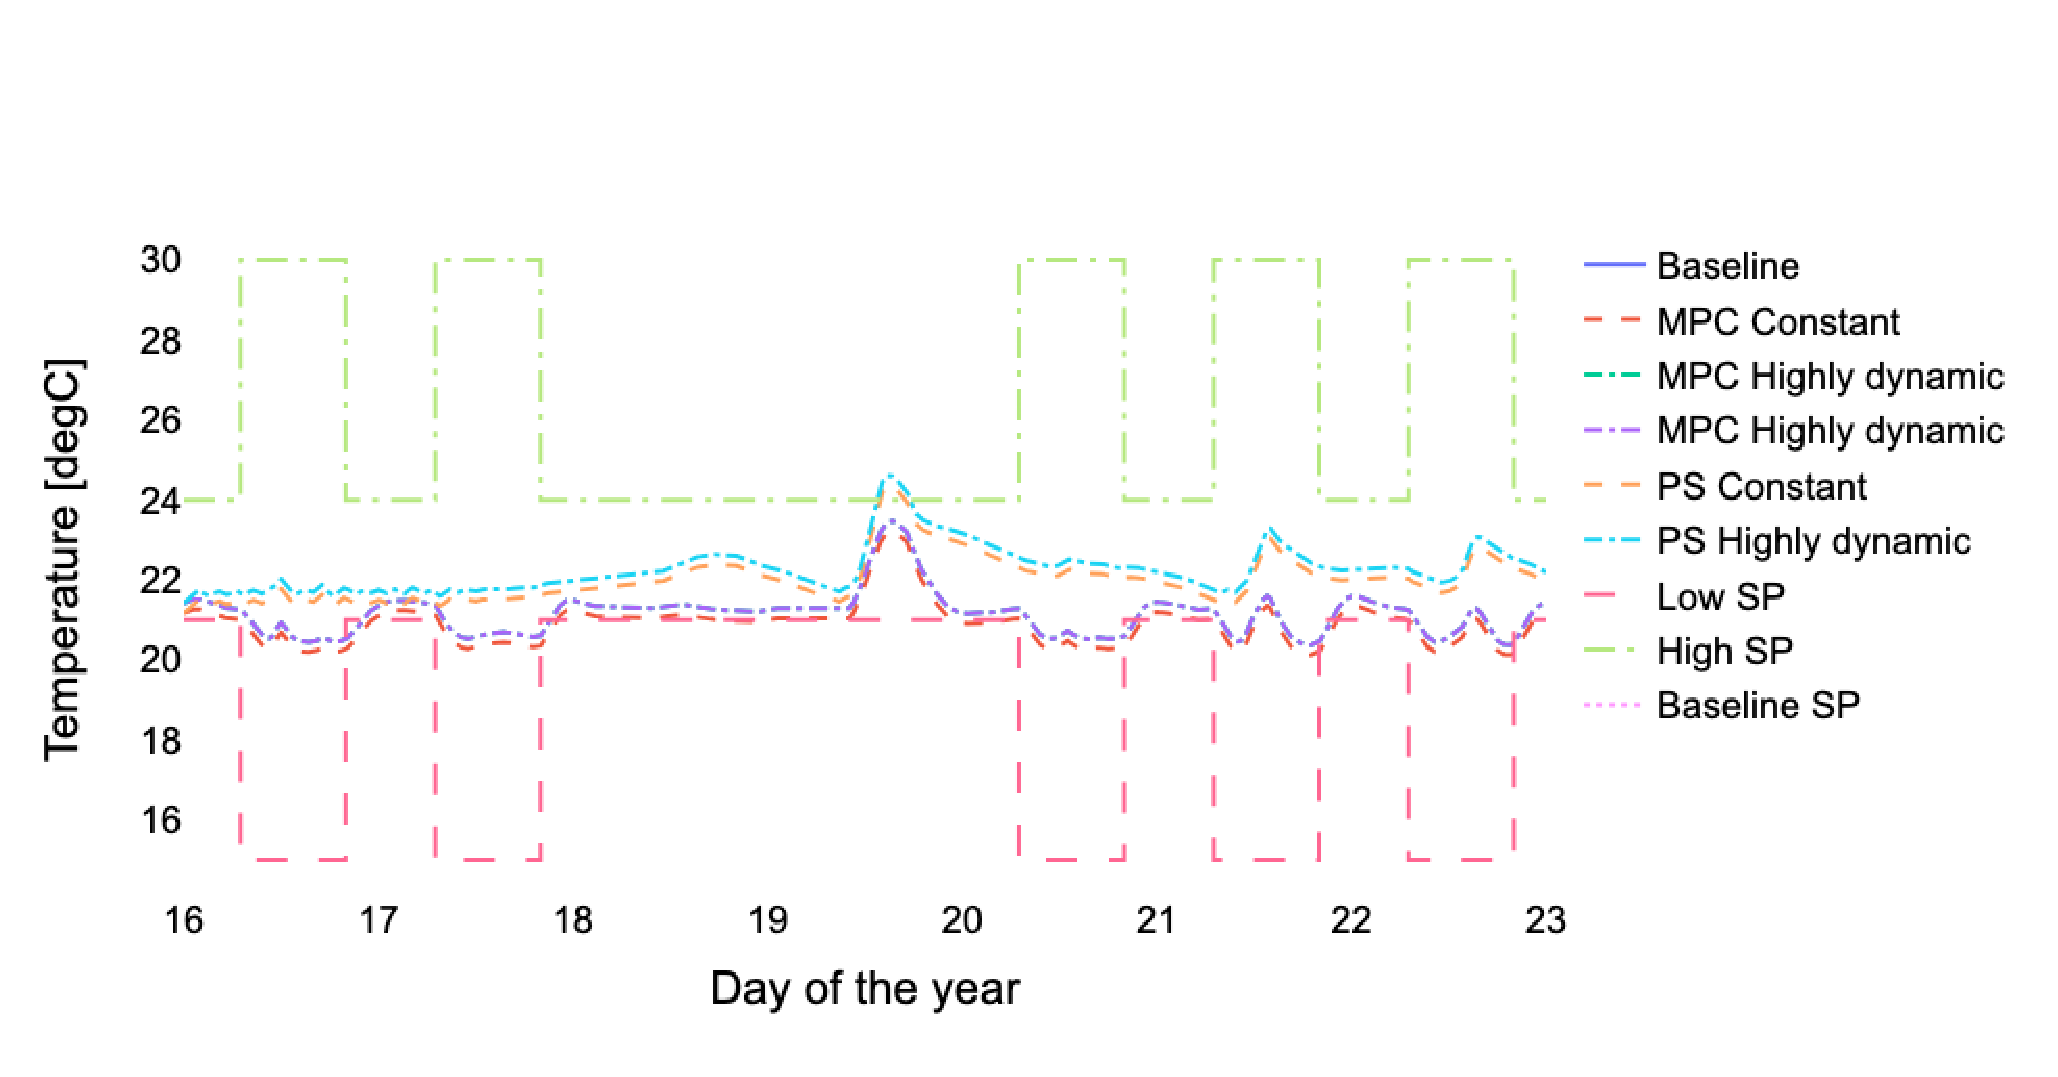
\includegraphics[width=\linewidth]{images/boptest/Fig4.eps}
% figure caption is below the figure
\caption{Indoor zone temperature through the simulation for the baseline, the MPC and program synthesis in \emph{peak heat period}, together with the lower and upper comfort limits and temperature setpoint for baseline controller.}
\label{fig:temp-peak}       % Give a unique label
\end{figure}

\paragraph{Typical heat period}
The second week from the typical heat day period was simulated for the baseline, the MPC and the program synthesis. Both the MPC and program synthesis were run for the three electricity price scenarios. As the baseline controller's logic is independent of the pricing scheme, its performance is not influenced by the prices, and thus just a simulation of the baseline controller is considered for each period. Table \ref{tab:3} depicts the KPI corresponding to each simulation.

\begin{table}
    \caption{Overview of KPI of each controller in the typical heat period.}
    \label{tab:3}
    
    \centering
    \begin{tabular}{lllllll}
        \hline
        \noalign{\smallskip}
        Controller & Price Scenario & Discomfort & Energy Use & Energy Cost & Emissions  \\
        & & [K·h/zone] & [kWh/m2] & [€/m2] & [kgCO2eq/m2] \\
        \noalign{\smallskip}
        \hline
        \noalign{\smallskip}
        Baseline & - & 4.385 & 1.766 & 0.448 & 0.295 \\
        MPC & Constant & 0.156 & 1.232 & 0.310 & 0.205 \\
        MPC & Dynamic & 0.148 & 1.224 & 0.312 & 0.205 \\
        MPC & Highly dynamic & 0.147 & 1.232 & 0.289 & 0.206 \\
        PS & Constant & 20.450 & 1.205 & 0.305 & 0.201 \\
        PS & Highly dynamic & 20.450 & 1.205 & 0.305 & 0.201 \\
        \noalign{\smallskip}
        \hline
    \end{tabular}
\end{table}

The MPC shows an overall improvement in the thermal comfort with respect to the baseline controller in the three scenarios, as well as a reduction in energy use, energy cost and CO2 emissions. The thermal discomfort decrease compared to the baseline is of 96.44\% for the constant price scenario, 96.62\% when the price is dynamic, and 96.65\% for highly dynamic prices. The energy use savings range between 30.23\%-30.7\%, the energy cost reduction is very similar, being 30.8\%, 30.36\% and 35.5\% for constant, dynamic and highly dynamic respectively. CO2 emissions reduction are also achieved, up to 30.16\% in the most favourable scenario.

In the case of program synthesis, the thermal discomfort is 78.56\% greater than with the baseline controller. On the other hand, the energy use reduction is up to 31.77\%, the energy cost is 31.91\% lower with program synthesis and the emissions are also 31.86\% lower.

The evolution of the indoor zone temperature along the simulation for the baseline controller, the MPC and program synthesis in the three price scenarios is shown in Figure \ref{fig:temp-peak}. The baseline setpoint is depicted, which is equal to 21.2ºC during occupation hours, and it is lowered to 20.2ºC when there are no occupants. The low and high limits that are used to calculate the thermal discomfort are also depicted in Figure \ref{fig:temp-typical}.

% For one-column wide figures use
\begin{figure}
  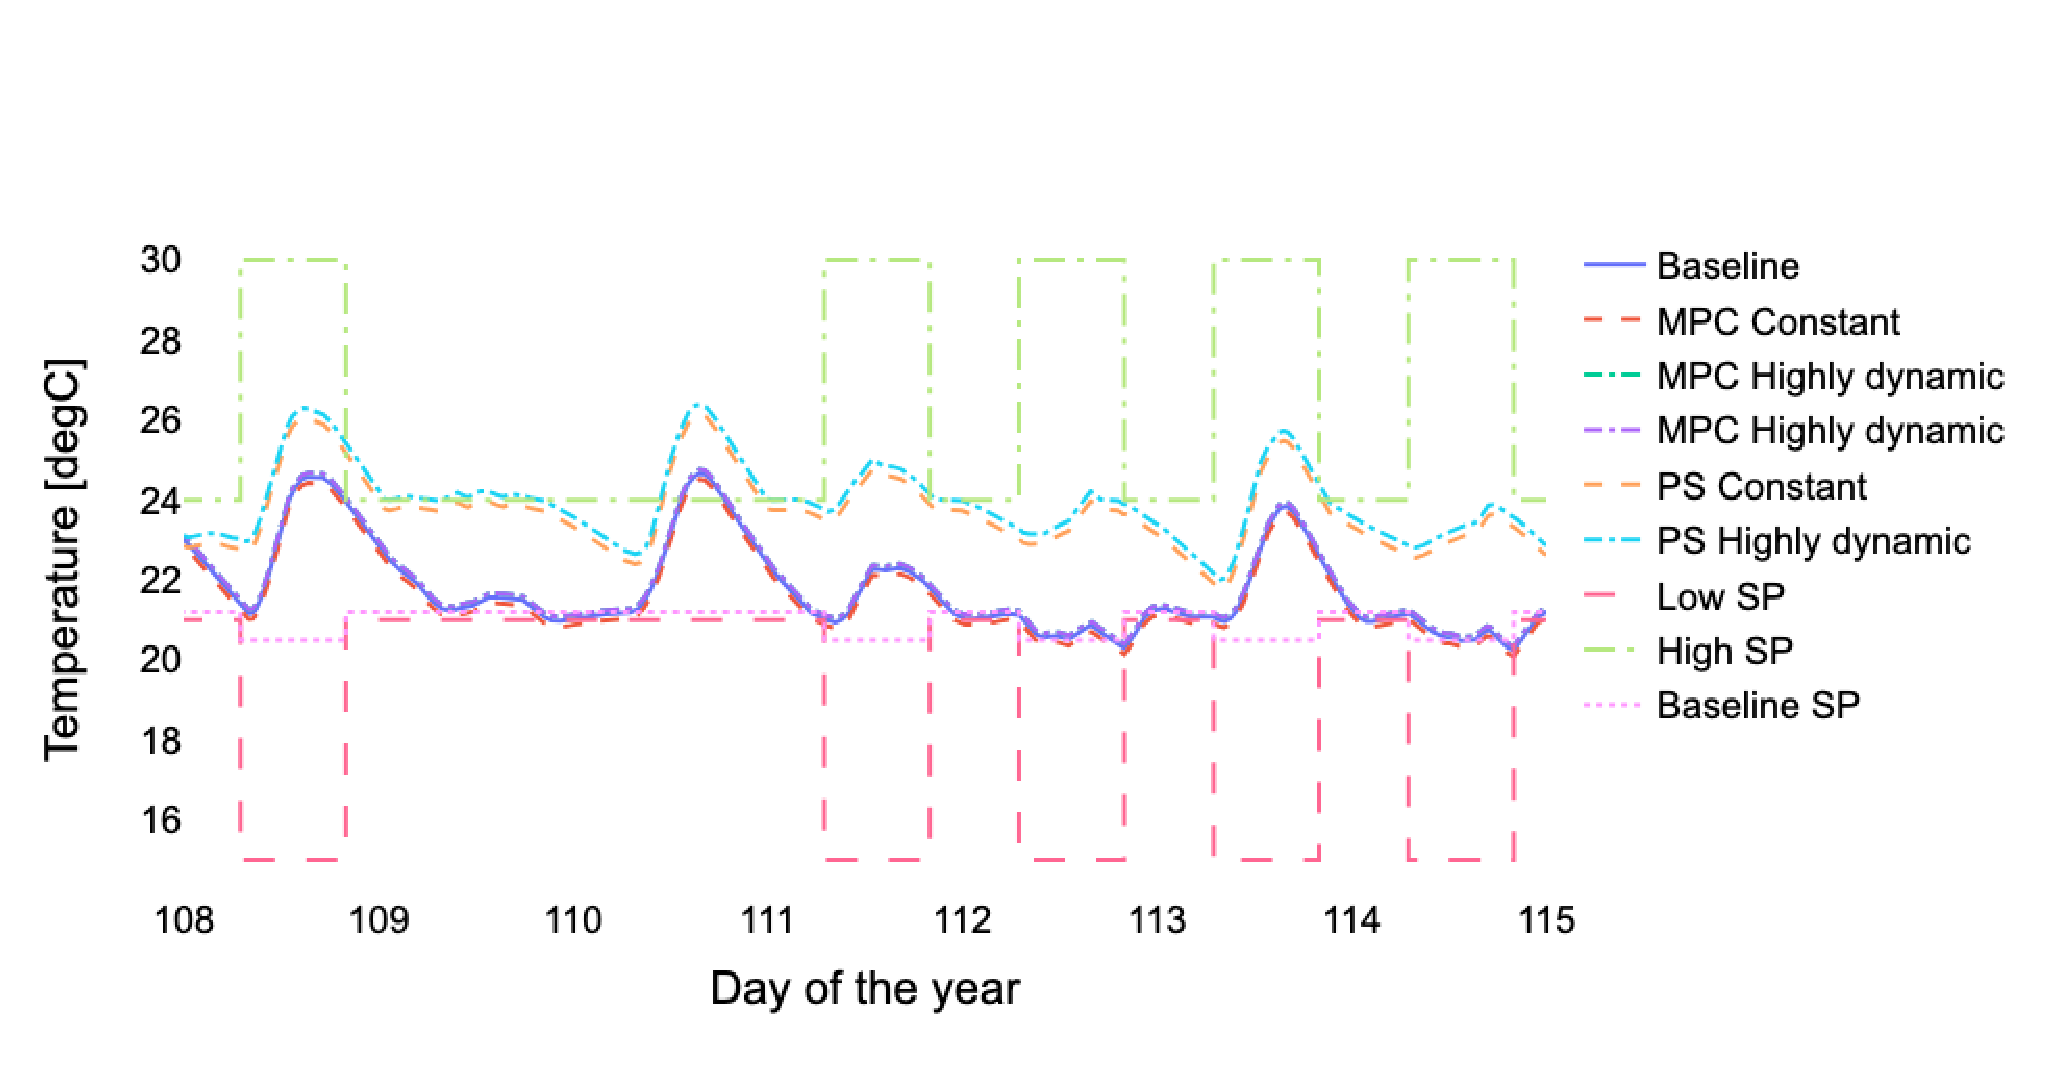
\includegraphics[width=\linewidth]{images/boptest/Fig7.eps}
% figure caption is below the figure
\caption{Indoor zone temperature through the simulation for the baseline, the MPC and program synthesis in \emph{typical heat period}, together with the lower and upper comfort limits and temperature setpoint for baseline controller.}
\label{fig:temp-typical}       % Give a unique label
\end{figure}